%%%%%%%%%%%%%%%%%%%%%%%%%%%%%%%%%%%%%%%%%%%%%%%%%%%%%%%%%%%%
%%%%%%%%%%%%%%%%%%%%%%%%%%%%%%%%%%%%%%%%%%%%%%%%%%%%%%%%%%%%
%%%%%%%%%%%%%%%%%%%%%%%%%%%%%%%%%%%%%%%%%%%%%%%%%%%%%%%%%%%%
\section{The Dune Workflow for Simulations with CAD-Models}\label{Sec:Workflow}
%%%%%%%%%%%%%%%%%%%%%%%%%%%%%%%%%%%%%%%%%%%%%%%%%%%%%%%%%%%%
%%%%%%%%%%%%%%%%%%%%%%%%%%%%%%%%%%%%%%%%%%%%%%%%%%%%%%%%%%%%
%%%%%%%%%%%%%%%%%%%%%%%%%%%%%%%%%%%%%%%%%%%%%%%%%%%%%%%%%%%%

%-------------------------------------------------------------------
\subsection{Overview}
% Bilder
% Tool Chain

\begin{frame}
  \frametitle<presentation>{Overview}
  \textbf{Real world problems can be defined on complex domains.}
  \begin{itemize}
    \item Often, such domains are given by CAD-models.
    \item Dune cannot handle such models directly.
    \item $\rightarrow$ Need of a workflow to import computational grids
      for CAD-models used in simulations.
  \end{itemize}
  The interface to meshed CAD-Models in Dune is via \lstinline!Gmsh!-files.
\end{frame}

\begin{frame}
  \frametitle<presentation>{Overview}
  The outline to import meshed CAD-models in Dune is
  \begin{enumerate}
    \item Create or retrieve a CAD-model.
    \item Edit and mesh the CAD-model with Gmsh
      \href{http://www.geuz.org/msh}{(www.geuz.org/gmsh)}.
    \item Export a \lstinline!.msh!-File from Gmsh.
    \item File can contain additional data such as connected subdomains.
    \item Import the mesh file with the \lstinline!Dune::GmshReader!.
    \item Evaluate physical data specified in the mesh file.
  \end{enumerate}
  The important steps will be shown in detail in the following sections.
\end{frame}

\begin{frame}
  \frametitle<presentation>{A Meshed CAD-Models Imported to Dune}
  The picture shows a sample geometry meshed with Gmsh on the left and the mesh
  imported by Dune on the right.
  %\begin{figure*}
  \begin{center}
    \includegraphics[width=0.48\textwidth]{./EPS/gcad3d_cyl_gmsh}  $\hspace{1mm}$
    \includegraphics[width=0.48\textwidth]{./EPS/gcad3d_cyl_dune}
    %\caption[]{Some example meshes import to Dune.}
    %\label{fig:CADExmapleMeshesToDune}
  \end{center}
  {\tiny (CAD-Model from gCAD3D).}
  %\end{figure*}
\end{frame}

\begin{frame}
  \frametitle<presentation>{The Workflow to Import meshed CAD-Models to Dune}
  In general we have the flow chart
  \begin{center}
    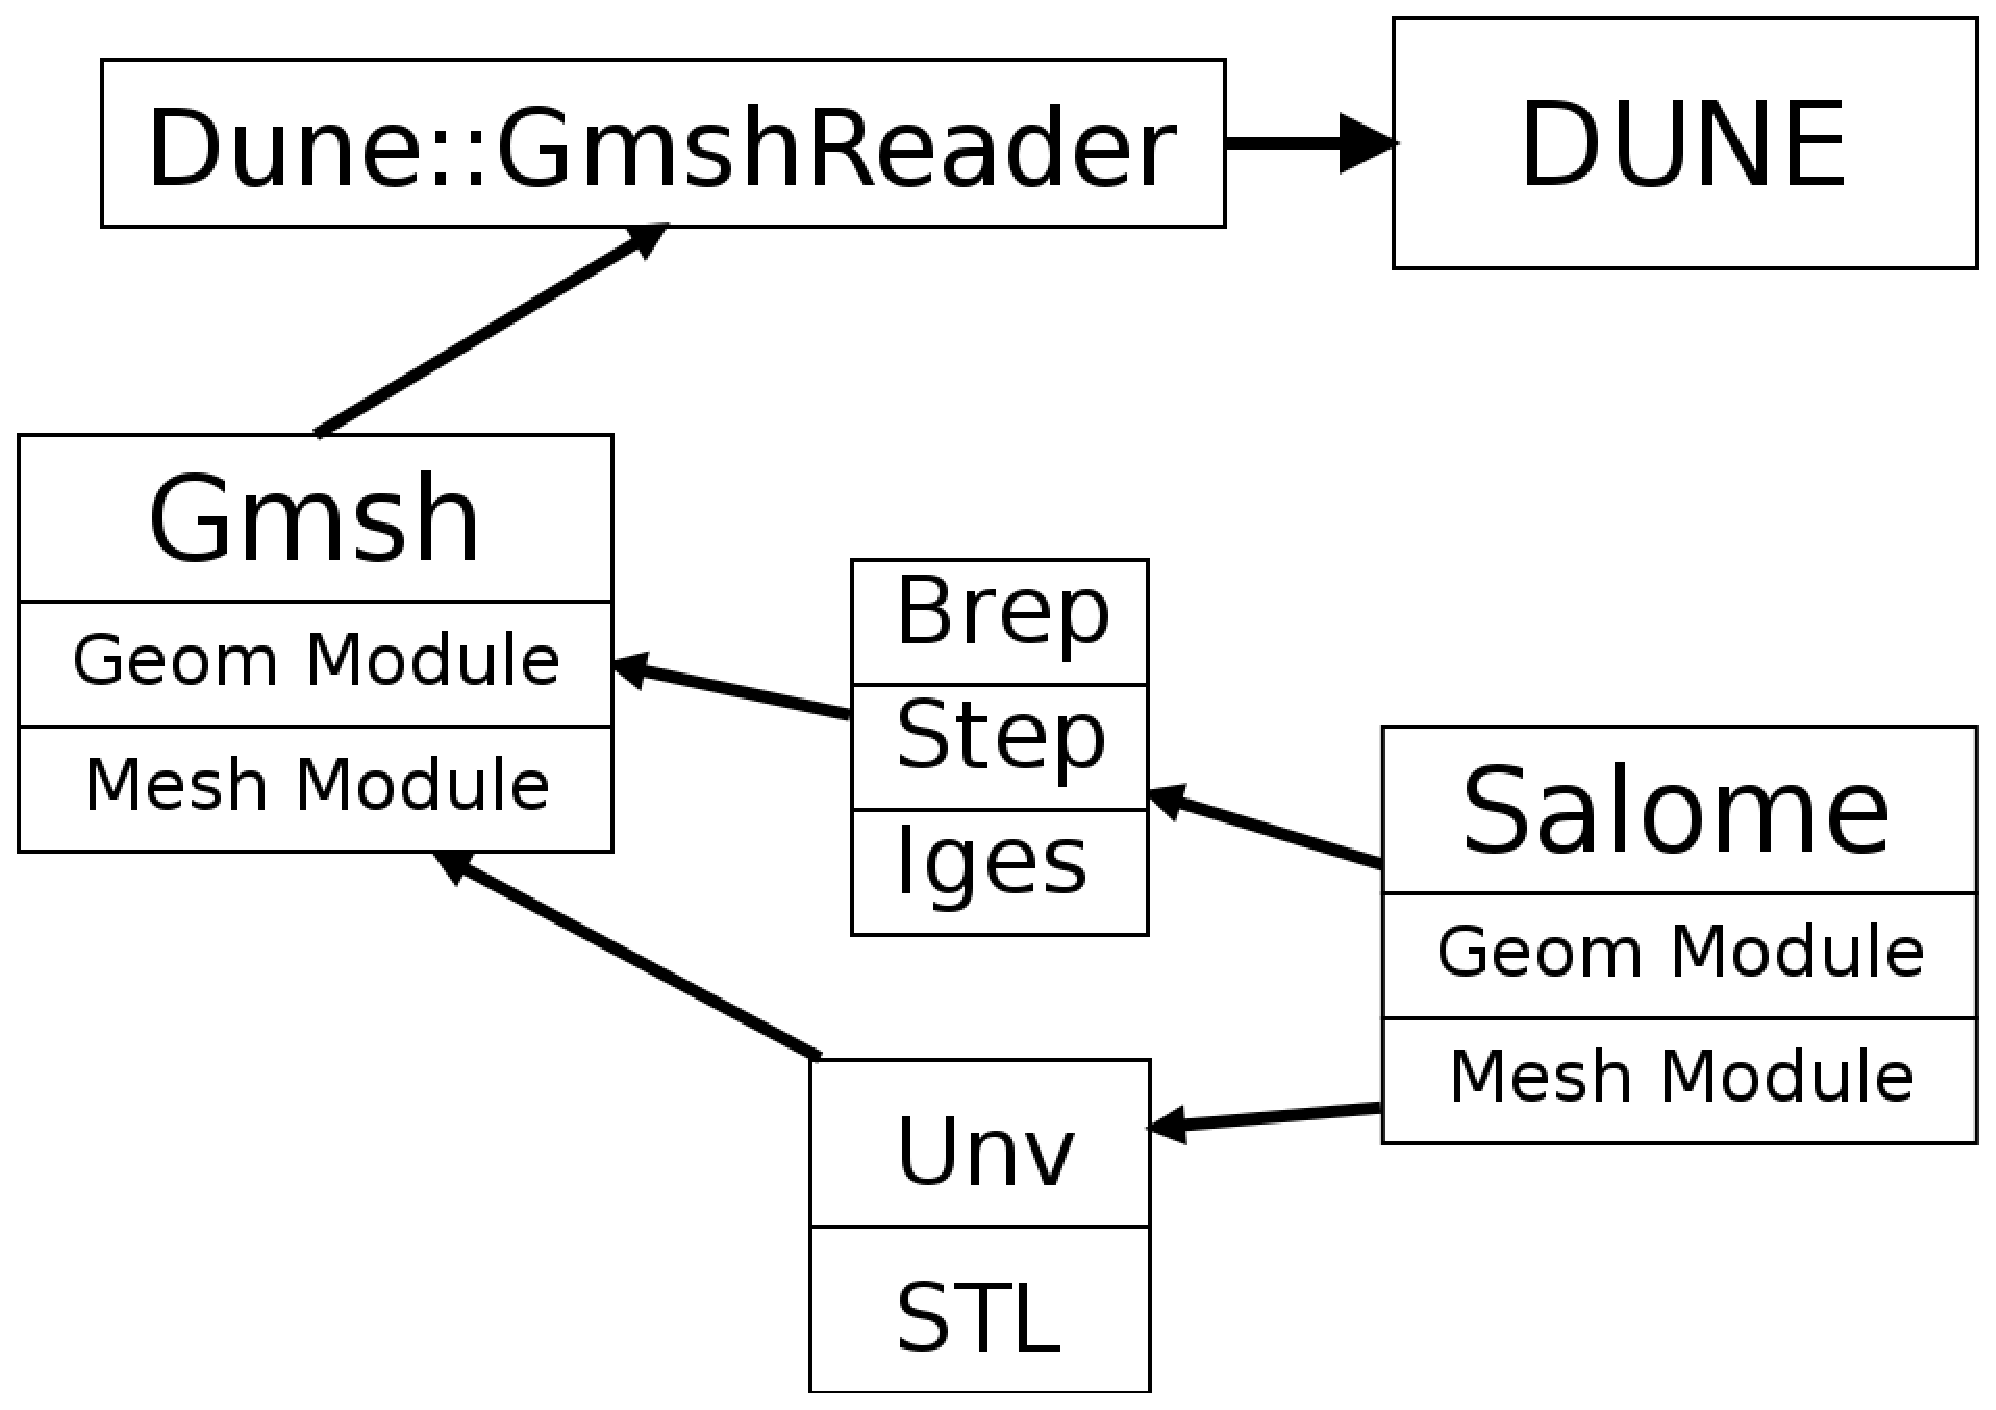
\includegraphics[width=0.7\textwidth]{./EPS/workflow}
  \end{center}
  Salome is another geometry modeller behind the Gmsh-Interface.
  Other tools might be applicable as well.
\end{frame}

%-------------------------------------------------------------------
\subsection{Gmsh and the DUNE Gmsh-Interface}
% Dune GmshReader
% Gmsh und OpenCascade
% Installation
% welche Grids?

\begin{frame}[fragile,allowframebreaks,allowdisplaybreaks]
  \frametitle{The Dune::GmshReader}
  We begin with the import of a Mesh file \lstinline!meshfile.msh! using Dune's
  \lstinline!GmshReader!:
  \lstinputlisting[basicstyle=\tiny,numbers=left,
      numberstyle=\tiny, numbersep=2pt]{./src_examples/gridtest.cc}
      \textbf{Changes to the code seen up to now are:}
  \begin{itemize}
    \item Include the Gmsh-Interface header from \lstinline!dune-grid! (line
      $12$).
    \item Use \lstinline!UGGrid! -- Up to now \lstinline!UGGrid! and
      \lstinline!ALUGrid! are feasible for Gmsh meshes (line $33$-$35$).
    \item Import gmsh file (line $37$-$40$).
  \end{itemize}
\end{frame}

\begin{frame}[fragile,allowframebreaks,allowdisplaybreaks]
  \frametitle{Gmsh}
  The mesh-files are created and exported by the exported software \emph{Gmsh},
  which is able to
  \begin{itemize}
    \item Import CAD models in various formats
      (\lstinline!GEO, STEP, IGES, BREP, ACIS, ...!),
    \item Group subdomains of the models into phyiscal \emph{entities} or
      \lstinline{groups},
    \item Mesh the models,
    \item Write the meshes including physical group regions to a mesh file
      (file-ending \lstinline!.msh!).
  \end{itemize}
  \pagebreak<presentation>
  It comes with a more or less user-friedly GUI:
  \begin{center}
    \includegraphics[width=0.7\textwidth]{./EPS/gcad3d_deckel}
  \end{center}
  {\tiny (CAD-Model from gCAD3D).}

  \textbf{Further features of Gmsh:}
  \begin{itemize}
    \item Geometry Kernel: OpenCascade
      \begin{itemize}
        \item Gmsh $\leq$ 2.3.1: Build from scratch for OpenCascde and Gsmh
          necessary to import CAD-models.
        \item Gmsh $\geq$ 2.4.2: Precompiled build for Linux and MAC work with
          OpenCascade packages from distributor (Tested for Debian and MacOS).
      \end{itemize}
    \item Does not cover full functionality of geometry kernel.
    \item Possible: Second order boundaries. Dune supports them (But there is a
      bug in the current trunk!).
  \end{itemize}
\end{frame}

%-------------------------------------------------------------------
\subsection{Importing and Meshing CAD-Geometries with Gmsh}
% CAD-Files Uebersicht
% install with opencascade
% Import
% Welcher Mesher?

\begin{frame}
  \frametitle{Common CAD-File Formats Readable by Gmsh}
  \textbf{Gmsh allows to import CAD-models in common formats:}
  \begin{center}
    \begin{tabular}{|l|l|l|}
      \hline
      Format & Ending & Description
      \\
      \hline
      \hline
      STEP & \lstinline!.stp, .step! & ISO10303 norm\\
      & & Able to save all data of work process
      \\
      \hline
      IGES & \lstinline!.igs, .iges! & Transfers mainly geometry data\\
      & & 2D/3D shape models (NURBS + Bezier)
      \\
      \hline
      ACIS & \lstinline!.sat! & Volume modelling kernel. Widely used format.
      \\
      \hline
      BREP & \lstinline!.brp! & List of convex polygons consisting of point lists\\
      & & In OpenCascade very limited!
      \\
      \hline
      GEO & \lstinline!.geo! & The native Gmsh geometry format.
      \\
      \hline
    \end{tabular}
  \end{center}
  Imported models are converted to the geo-format internally. Gmsh's merge
  function preserves the original format.
\end{frame}

\begin{frame}
  \frametitle{Meshing CAD-Models with Gmsh}
  \textbf{Gmsh comes with a meshing functionality:}
  \begin{enumerate}
    \item Advancing front, and
    \item Delaunay meshes.
    \item Mesher can be parametrized by hypothesises.
    \item All meshes handled as unstructured grids.
    \item Only simplicial meshes.
  \end{enumerate}
\end{frame}

\subsubsection*{Further notes on ineraction between Dune and Gmsh}

\begin{frame}
  \frametitle{Dune and Gmsh Notes}
  \begin{enumerate}
    \item In Dune: Higher order elements available!
    \item But meshes from Gmsh are always linear
      (though boundary segment apprximation might be quadratic).
    \item Dune Grids from Gmsh Meshes created with \emph{GridFactories}.
      \begin{itemize}
        \item GridFactory implementation depends on Dune GridType.
        \item For UG and ALU the Factories are ready.
      \end{itemize}
  \end{enumerate}
\end{frame}

%-------------------------------------------------------------------
\subsection{Attaching Data to a CAD-Geometry and its Mesh}
% Gruppen in Gmsh
% Gmshreader nur eine Gruppe pro Element!
% PDELab-Code

\begin{frame}[fragile,allowframebreaks,allowdisplaybreaks]
  \frametitle<presentation>{Physical Groups in CAD-Models}
  \textbf{Physical parameters can be associated to subdomains of the
  domain, e.g.}
  \begin{itemize}
    \item Material properties (conductivities,\ldots),
    \item Boundary conditions,
    \item \ldots
  \end{itemize}
  \textbf{The subdomains available in Gmsh are:}
  \begin{itemize}
    \item Volume groups,
    \item Surface groups,
    \item Line groups,
    \item Point groups.
  \end{itemize}
  %\pagebreak<presentation>
  %\textbf{Physical groups can be set by user interaction:}
  %\begin{center}
  %  \includegraphics[width=0.6\textwidth]{./EPS/crank/geo2}
  %\end{center}
  %The meaning of the numbers will be explained forthwith.
\end{frame}

\begin{frame}
  \frametitle<presentation>{Evaluating Physical Groups with the Dune::GmshReader}
  The \lstinline!Dune::GmshReader! is able to read
  \begin{itemize}
    \item Volume groups, and
    \item Surface groups
  \end{itemize}
  from a \lstinline!.msh!-file. Mappings
  \begin{itemize}
    \item Codim 0 entities $\Leftrightarrow$ Geometry volume groups, and
    \item Codim 1 entities $\Leftrightarrow$ Geometry surface groups,
  \end{itemize}
  can be saved in two \lstinline!std::vector<int>!s.
\end{frame}

\begin{frame}[fragile,allowframebreaks,allowdisplaybreaks]
  \frametitle<presentation>{An Example for Physical Grouping in Gmsh}
  \textbf{The next pictures show how physical groups can be set by user interaction in
  Gmsh:}
  \begin{center}
    \includegraphics[width=0.8\textwidth]{./EPS/L/L_numbers_vols_faces}
  \end{center}
  Volumes and Faces of geometry models have unique numbers. Here: Volume numbers --
  yellow, surface -- grey. This model has internal faces.
  \begin{center}
    \includegraphics[width=0.8\textwidth]{./EPS/L/L_volgroup1}
  \end{center}
  The model volume consists of several sub-volumes which we divide into two
  physical groups. This is the first one\ldots
  \begin{center}
    \includegraphics[width=0.8\textwidth]{./EPS/L/L_volgroup2}
  \end{center}
  \ldots and this the second.
  \begin{center}
    \includegraphics[width=0.8\textwidth]{./EPS/L/L_surfgroup1}
  \end{center}
  Next we create two surface groups. Group $1$\ldots
  \begin{center}
    \includegraphics[width=0.8\textwidth]{./EPS/L/L_surfgroup2}
  \end{center}
  \ldots and group $2$. Internal faces are not grouped.
  \begin{center}
    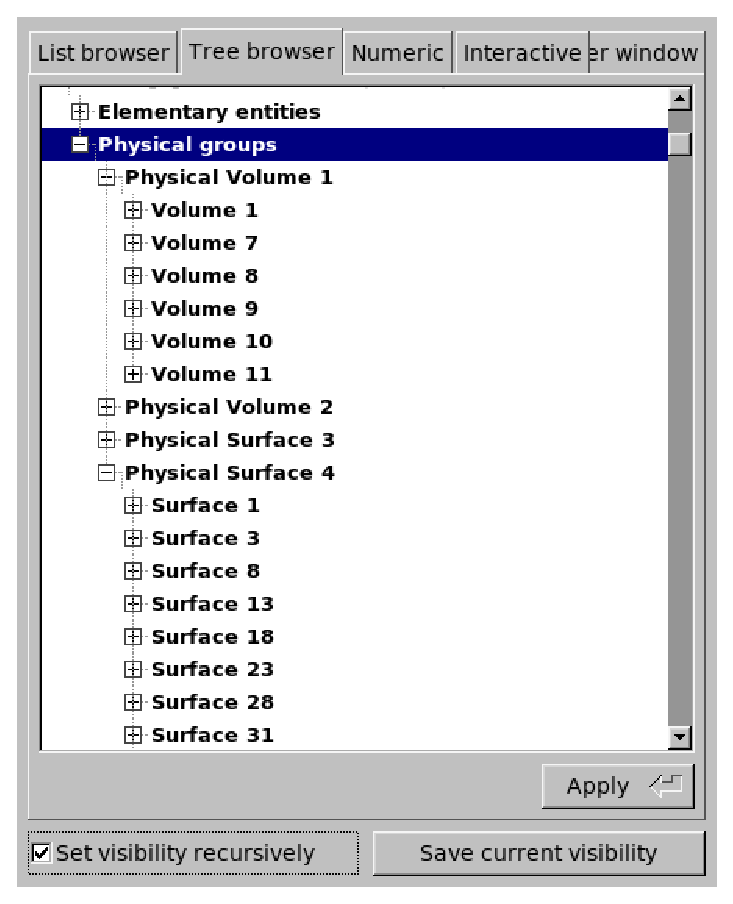
\includegraphics[width=0.355\textwidth]{./EPS/L/L_physgroups}\rule{1mm}{0mm}
    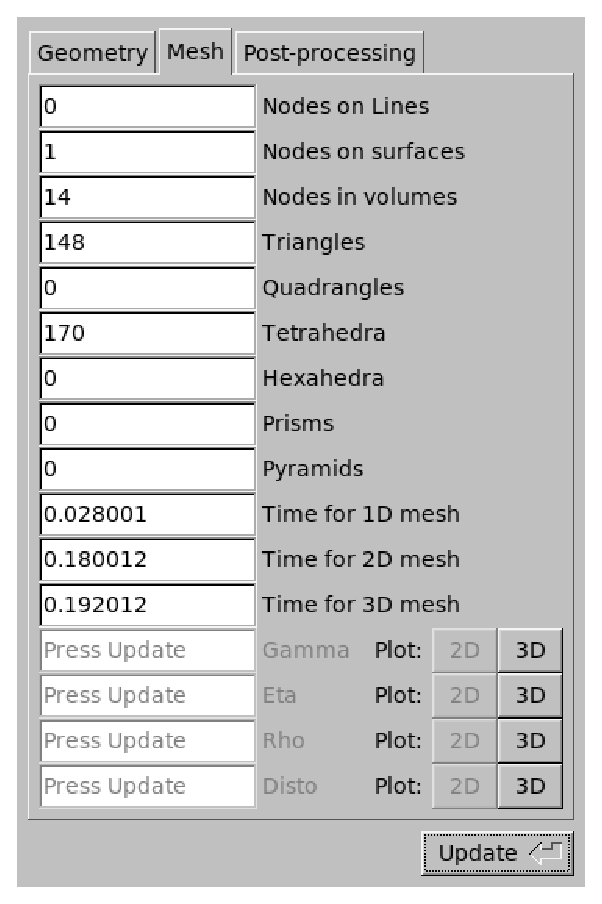
\includegraphics[width=0.29\textwidth]{./EPS/L/L_meshstatistics}\rule{1mm}{0mm}
    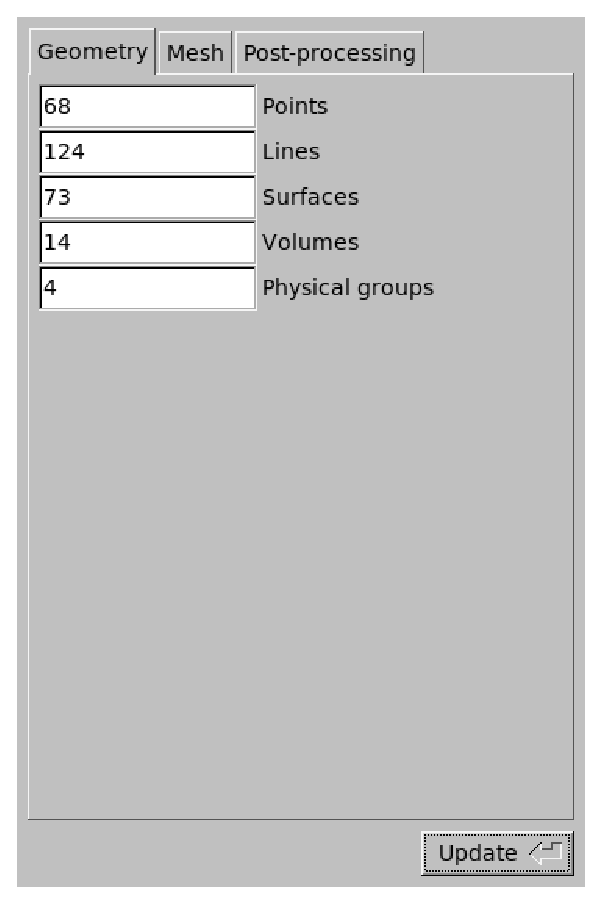
\includegraphics[width=0.29\textwidth]{./EPS/L/L_geostatistics}\\
  \end{center}
  This picture shows physical grous, mesh and geo statistics.
\end{frame}

%-------------------------------------------------------------------
\subsection{A sample Dune-Simulation importing a CAD-model}

\begin{frame}<presentation>[fragile,allowframebreaks,allowdisplaybreaks]
  \frametitle{Using Physical Groups from within Dune}
  \textbf{Next we show how the physical groups can be used in Dune. We use the
  examples from the stationary problems section. Changes are}:
  \begin{itemize}
    \item Use \lstinline!Dune::GmshReader!,
    \item Use \lstinline!UGGrid!,
    \item Use $P1$-elements for simplicity only,
    \item Rewrite
      \begin{itemize}
        \item \lstinline!bctype.hh!,
        \item \lstinline!bcextension.hh!,
        \item Source term evaluation,
        \item Diffusion parameter evaluation.
      \end{itemize}
      \textbf{Boundary conditions and material parameters depend on the physical group
      maps now!}
    \item The PDELab local operator is parametrized with boundary selection and value
      classes, source term class and a class for the non-constant material
      parameter.
  \end{itemize}
  \textbf{The Code constist of four files:}
  \begin{itemize}
    \item \lstinline!e02.cc!: main file creating grid files from Gmsh files,
    \item \lstinline!e02_parameter.hh!: Parameter classes containg maps to
      physical groups,
    \item \lstinline!e02_P1.hh!: Set up the P1 driver,
    \item \lstinline!e02_operator.hh!: local operator parametrized by the
      classes from \lstinline!e02_parameter.hh!
  \end{itemize}
\end{frame}

\begin{frame}<presentation>[fragile,allowframebreaks,allowdisplaybreaks]
  \frametitle<presentation>{The Main File of the Example}
  \lstinputlisting[basicstyle=\tiny,numbers=left,
      numberstyle=\tiny, numbersep=2pt]{./src_examples/e02.cc}
  \textbf{Notes:}
  \begin{itemize}
    \item In line $80$, the \lstinline!GmshReader! takes two vectors
      (instantiated in lines $74,75$) to store volume and surface map data from
      the Gmsh file.
    \item In line $98-108$, the parameter classes for the problem are created.
      In the constructor they take the according vector. Example:
      \lstinline!LeiffelBCType! evaluates mapping \lstinline!Dune::Intersection!
      with boundary and physical group of geometry boundary.
    \item All parameter objects are passed to the driving function
      \lstinline!e02_P1! in line $111$ which forwards them to the operator.
  \end{itemize}
\end{frame}
\mode<article>{
  \begin{Lst} \mbox
  \nopagebreak
  \lstinputlisting[basicstyle=\scriptsize,numbers=left,
      numberstyle=\tiny, numbersep=2pt]{./src_examples/e02.cc}
  \end{Lst}
}

\begin{frame}<presentation>[fragile,allowframebreaks,allowdisplaybreaks]
  \frametitle<presentation>{The Parameter Class File of the Example}
  \lstinputlisting[basicstyle=\tiny,numbers=left,
      numberstyle=\tiny, numbersep=2pt]{./src_examples/e02_parameter.hh}
  \textbf{Notes:}
  \begin{itemize}
    \item The parameter classes evaluate the physical maps instead of global
      coordinates now!
    \item E.g., take the diffusion coefficient. Based on the element index
      it evaluates the physical grou map for volumes.
    \item Similar evaluates hold true for the other parameter classes.
  \end{itemize}
\end{frame}
\mode<article>{
  \begin{Lst} \mbox
  \nopagebreak
  \lstinputlisting[basicstyle=\scriptsize,numbers=left,
      numberstyle=\tiny, numbersep=2pt]{./src_examples/e02_parameter.hh}
  \end{Lst}
}

\begin{frame}<presentation>[fragile,allowframebreaks,allowdisplaybreaks]
  \frametitle<presentation>{The Driver function for the Example}
  \lstinputlisting[basicstyle=\tiny,numbers=left,
      numberstyle=\tiny, numbersep=2pt]{./src_examples/e02_P1.hh}
  \textbf{Notes:}
  \begin{itemize}
    \item The driver is nearly unchanged to the stationary examples.
    \item Passes the parameter objects to the operator and constraints.
  \end{itemize}
\end{frame}
\mode<article>{
  \begin{Lst} \mbox
  \nopagebreak
  \lstinputlisting[basicstyle=\scriptsize,numbers=left,
      numberstyle=\tiny, numbersep=2pt]{./src_examples/e02_P1.hh}
  \end{Lst}
}

\begin{frame}<presentation>[fragile,allowframebreaks,allowdisplaybreaks]
  \frametitle<presentation>{The Parametrized Local Operator for the Example}
  \lstinputlisting[basicstyle=\tiny,numbers=left,
      numberstyle=\tiny, numbersep=2pt]{./src_examples/e02_operator.hh}
  \textbf{Notes:}
  \begin{itemize}
    \item The operator is now parametrized with the boundary type selection,
      boundary extension and boundary flux classes.
    \item Source term vanishes but could also be a paramter to the operator.
    \item Evaluation of the parameter in operator via enities and intersecions.
      Compare the parameter classes!
  \end{itemize}
\end{frame}
\mode<article>{
  \begin{Lst} \mbox
  \nopagebreak
  \lstinputlisting[basicstyle=\scriptsize,numbers=left,
      numberstyle=\tiny, numbersep=2pt]{./src_examples/e02_operator.hh}
  \end{Lst}
}

%-------------------------------------------------------------------
\subsection{Salome and some other Open Source CAD-Tools}

% Constructing Geometries
% Export von geo und unv
% Ausblick: Reader
\begin{frame}
  \frametitle{Salome}
  \textbf{Salome is a more user-friendly CAE-environment which can also export
  CAD-models and meshes suitable for Gmsh-Import}.
  \begin{itemize}
    \item Geometry Kernel: OpenCascade, exposes more of the functionality than Gmsh.
    \item Can import and export IGES-, STEP-, BREP-, ACIS-files.
    \item Can import and export STL and UNV-meshes.
    \item Has a generic Mesher interface (Available: Netgen, GHS3D, ...)
    \item User friendly GUI for creating and processing CAD-models.
  \end{itemize}
\end{frame}

\begin{frame}
  \frametitle{Other Open Source CAD-Tools}
  %\begin{table}
    Some other CAD-Tools which are able to export geometry models or mesh
    files suitable for Gmsh import:
    \begin{center}
      \small
      \begin{tabular}{|c|c|c|c|c|c|}
        \hline
        Tool & Licence & Geom & Geom & Mesh
        \\
        &  & Import & Import & Export
        \\
        \hline
        \hline
        Gmsh & LGPL & geo & iges, step, brep, acis &
        \\
        \hline
        Salome & LGPL & iges, step, brep, acis & iges, step, brep, acis & unv,
        stl
        \\
        \hline
        BRLCad & GPL &  &  &
        \\
        \hline
        gCAD3D & Freeware & step, iges & step, iges &
        \\
        \hline
        Blender & own (BL) & CSG & iges &
        \\
        \hline
        PythonOCC & GPL & &  &
        \\
        \hline
      \end{tabular}
      %\caption{Some CAD tools.}
      %\label{tab:CADTools}
    \end{center}
  %\end{table}
\end{frame}

\cleardoublepage
